\begin{document}
  \subsection*{Hardware}
  
  While developing this project, an agile-like methodology was adopted.
  Each two week sprint ended with a review of what had been done towards the project and what would be done in the next sprint.
  Focus shifted from sprint to sprint but each had to produce something useable towards the final product.
  Keeping track of tasks in each sprint and between sprints was made easier with tools such as Trello which uses the Kanban system for organising tasks.

  In the earlier sprints, the focus was on understanding each of the components that would be used in the final product.
  As well as gaining understanding, the early sprints were also used to produce code blocks that could be utilised in the final code build.
    Later sprints looked at assembling what was learnt into the final circuit.
  Figure \ref{fig:one} shows one of the first designs for the circuit taken from an early sprint, there are a number of issues in this design that will now be discussed before looking at the final design to show the changes that were made throughout the development cycle.
  This initial design shows the LCD, keypad, piezoelectric speaker and LED all wired to the Arduino Uno.
  This design didn't include the servo motor required by the design specification as there weren't enough digital I/O pins to support it.
  Other issues with this design included the use of digital pins zero and one.
  Using pins zero and one can cause an issue where, during the flashing process, the program counter becomes de-synchronised, this is caused by the tiny amount of resistance of the wires being in pins zero and one.
  The wires could be removed each time the Arduino's memory is written to but this later became more difficult as larger numbers of wires were added to the system.
  In a later version, it was decided to remove the use of pins zero and one to completely avoid this issue.
  The initial design also included only one LED, which was okay but to allow for better indication of what state the system is in, there was a need for more LEDs of different colours.
 \begin{figure}[h]
    \vspace{0.3cm}
    \begin{center}
      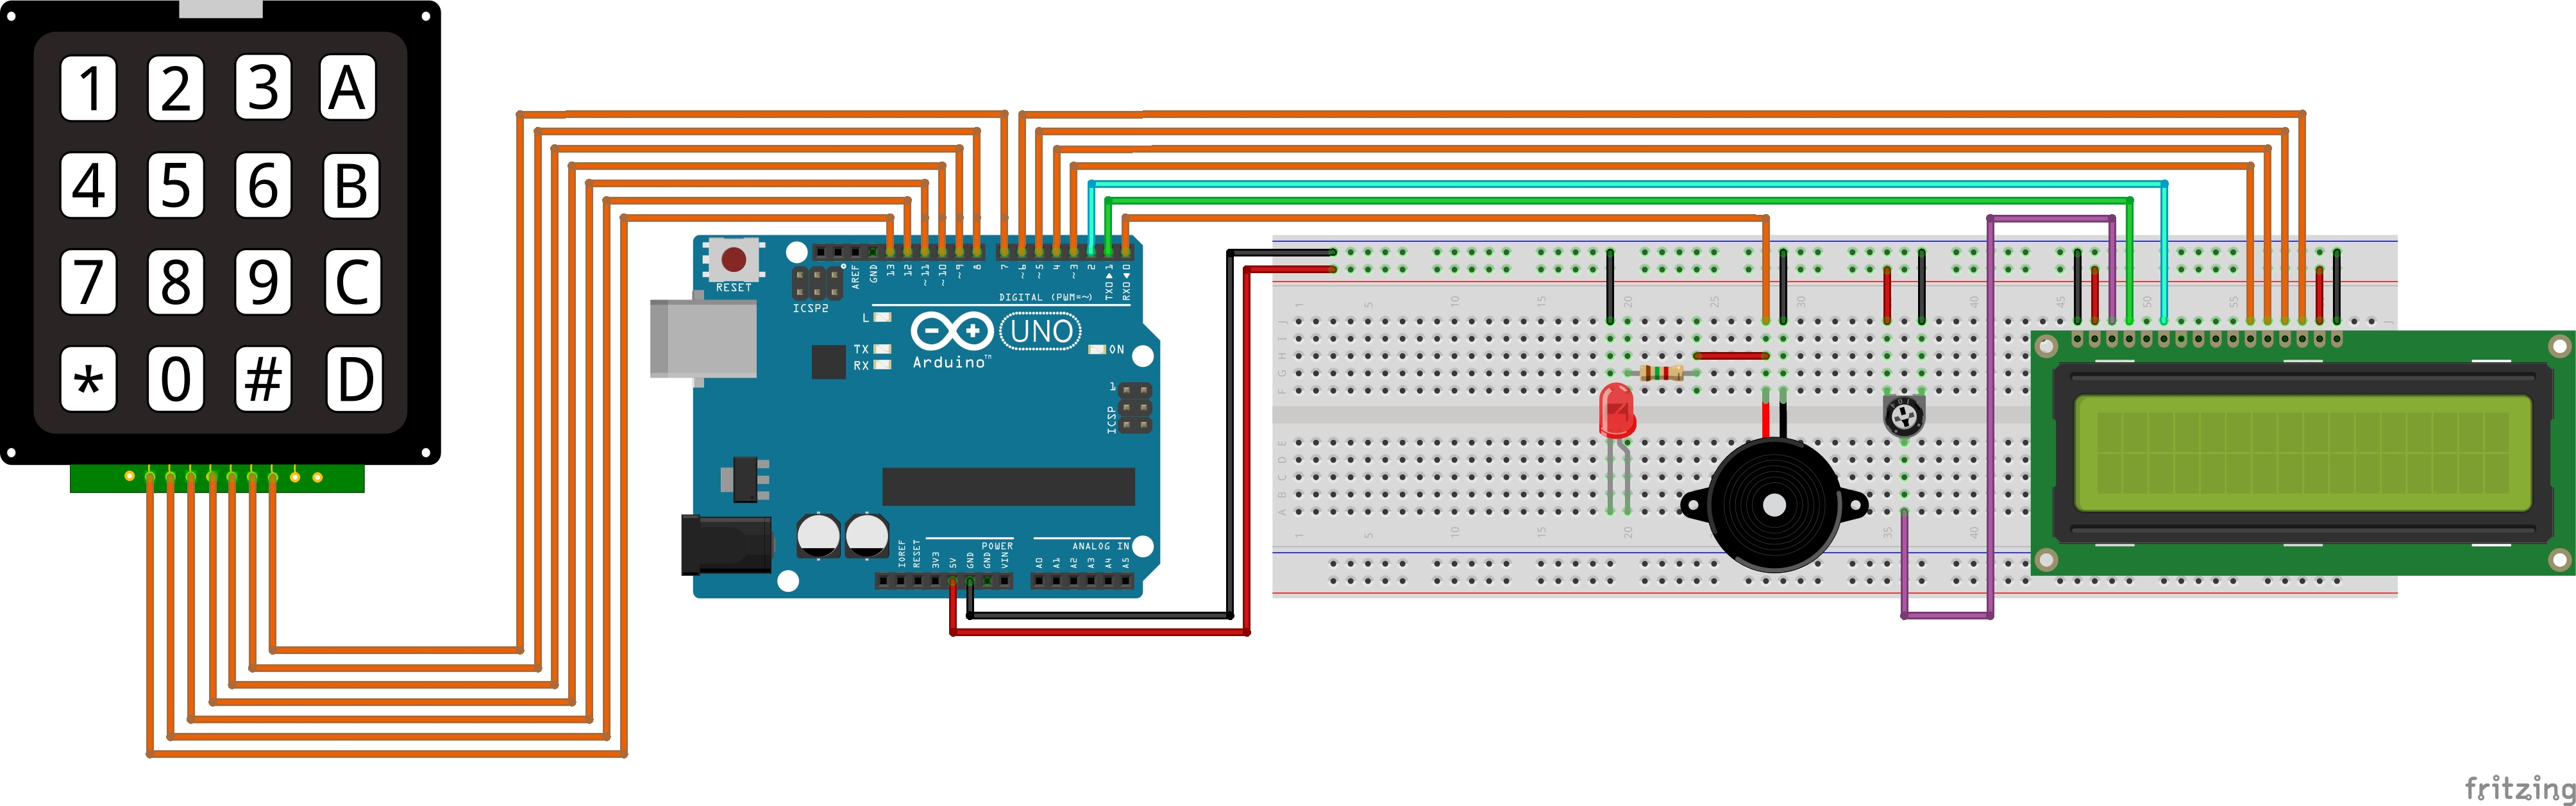
\includegraphics[width=0.68\textwidth]{initial.jpg}
    \end{center}
    \vspace{-20pt}
    \caption{Initial design using Fritzing}
    \label{fig:one}
    \vspace{0.3cm}
  \end{figure}

    The final design reached sought to correct each of these issues, Figure \ref{fig:two} shows the final design.
  The largest change from the initial design is that the LCD is no longer directly connect to the Arduino.
  Instead, the Arduino connects to a 74HC595N shift register which then connects to the LCD.
  lastminuteengineers (no date), sates that the [shift register] essentially controls eight separate output pins, using only three input pins.
  Normally, the LCD requires seven connections to the data pins on the Arduino, using the shift register allows for the LCD to be controlled using only three digital I/O pins.
  This means four more connections can be made to the Arduino while losing no functionality and freeing up digital I/O pins zero and one.
  The digital I/O pins used by the shift register had to be pins nine, eleven and thirteen, as these are the digital I/O pins that provide the Serial Peripheral Interface (SPI).
  SPI is a synchronous serial communication method, which the shift register requires in order to send the data correctly onto the LCD.
  Getting the shift register to work with the LCD also meant using a modified LCD header file provided by Juan Hernandez (Hernandez, 2016). 
    The final design also makes use of multiple LEDs which are connected to the piezoelectric speaker's and the servo motor's digital I/O pin as well.
  This means that by carefully controlling when the piezoelectric speaker is used, the red LED will light up and when the servo motor is used, the green LED will light up.
  An RGB LED was originally planned to be used, but due to a wiring error, the LED was damaged and couldn't be used in the final product.

  As was mentioned in the previous paragraph, the servo motor was also implemented in the final design using the extra digital I/O pins available.
  The servo motor is used to open and close the lock in the door, it is controlled by the Arduino and when the correct code is entered on the key pad, then the servo motor will open.
  The keypad, in both the initial and final design isn't fully connected.
  The right most column (containing the buttons A, B, C and D) is not connected, this is to free more I/O pins to be left available for other components. 
      \begin{figure}[h]
        \vspace{0.3cm}
        \begin{center}
        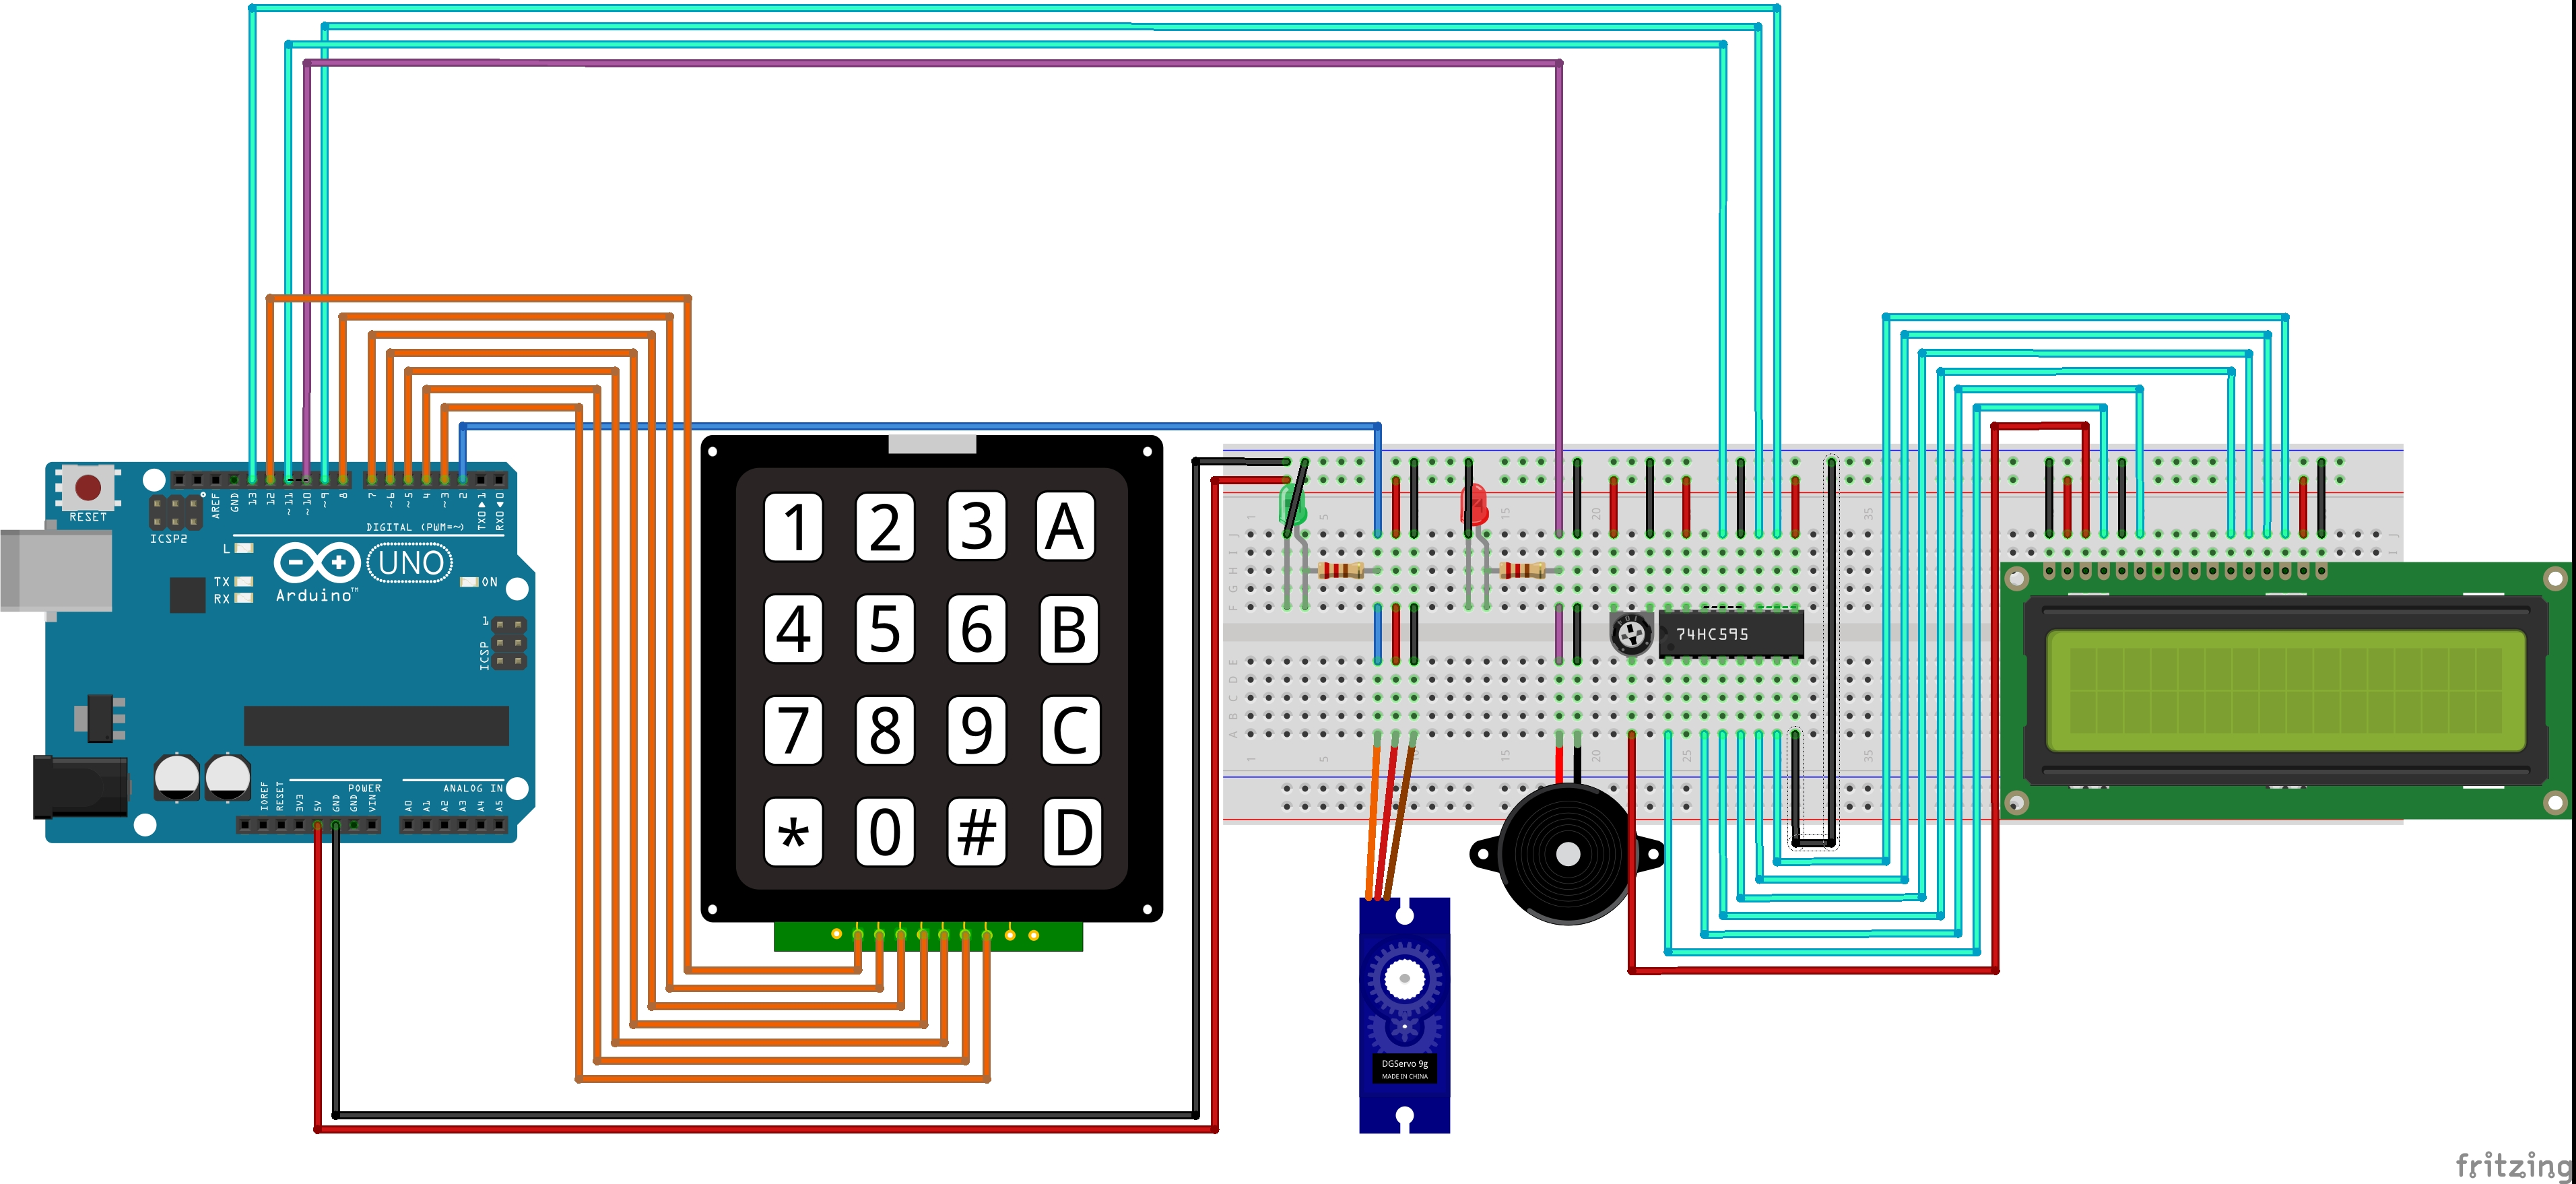
\includegraphics[width=0.68\textwidth]{final.jpg}
        \caption{Final design using Fritzing}
        \label{fig:two}
        \end{center}
        \vspace{0.3cm}
      \end{figure}

  \newpage

  \begin{figure}[h]
    \begin{center}
    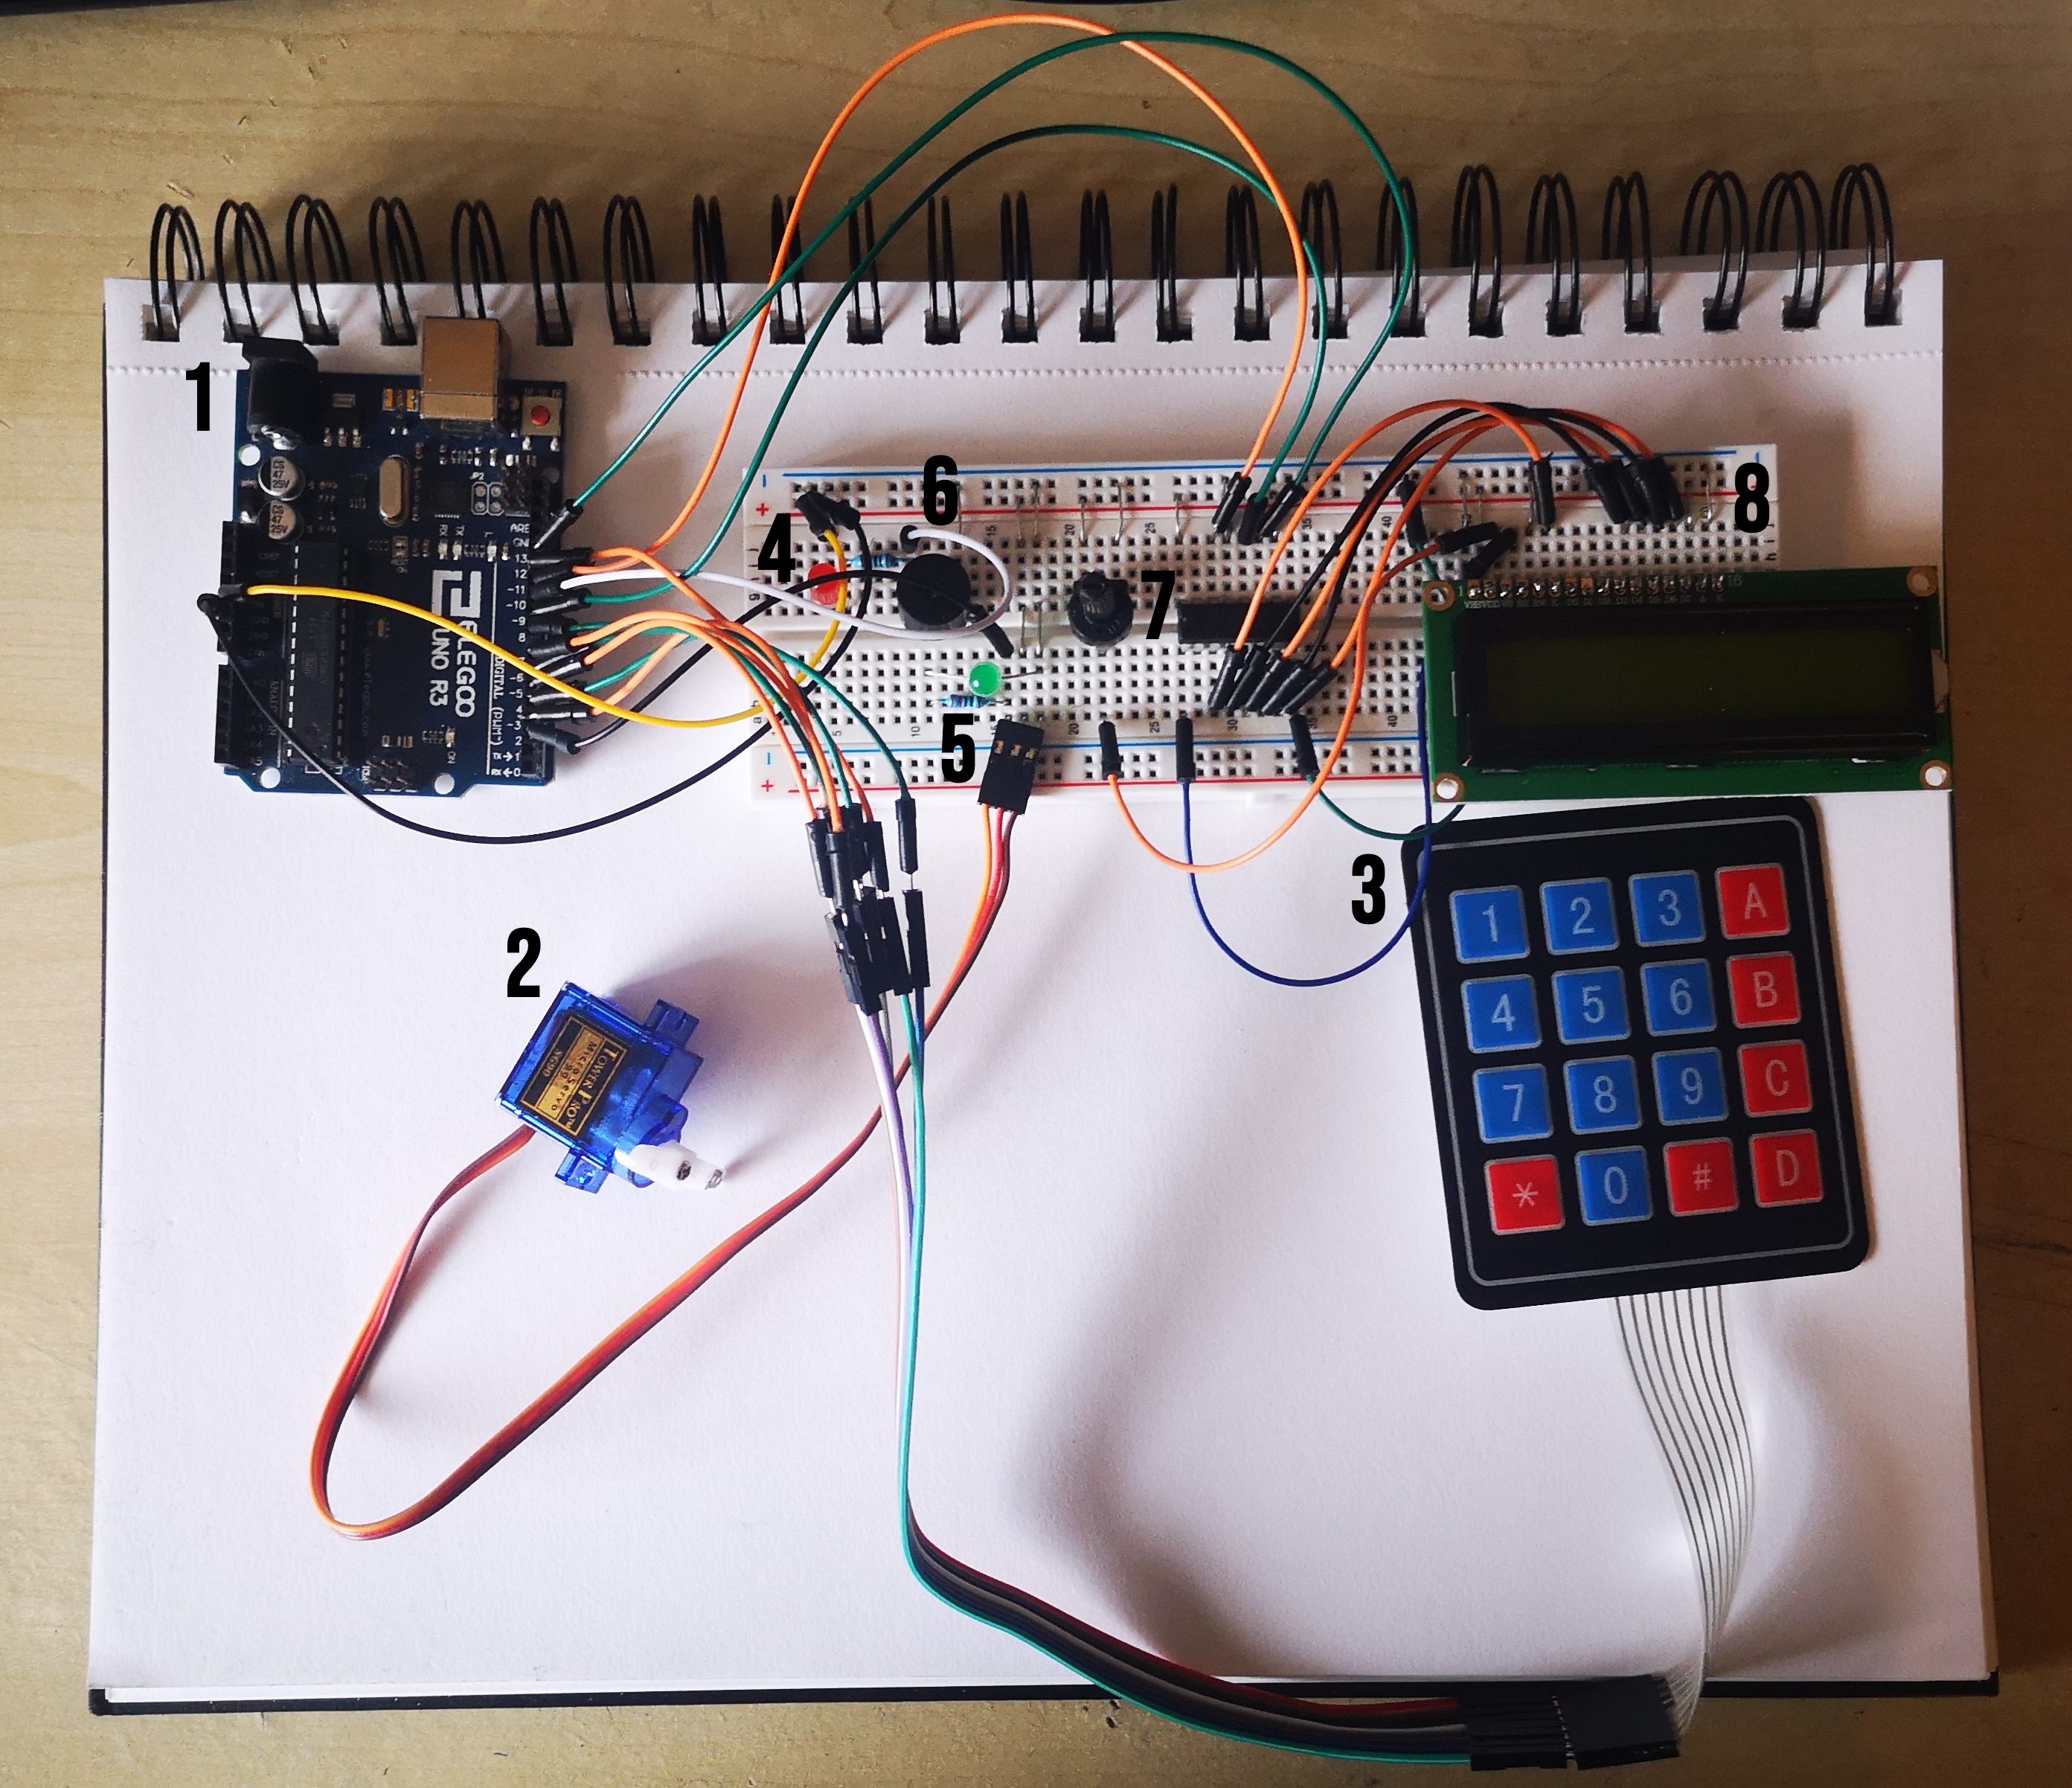
\includegraphics[width=0.8\textwidth]{labelled.jpg}
    \caption{Labelled circuit of the final design}
    \end{center}
  \end{figure}
  \begin{enumerate}
  \item Arduino Uno
  \item Servo Motor
  \item Keypad
  \item Red LED
  \item Green LED
  \item Piezoelectric Speaker
  \item 74HC595 Shift Register
  \item LCD
  \end{enumerate}
  \subsection*{Software}
  When developing the software for the project, it was decided early on to use heap allocated arrays to store the codes entered by the user.
  This choice allowed for better control of when and where memory was allocated and de-allocated, this is important as Guyer and Helbling (2016) note, typically [the Arduino has] 32 KB of flash memory for the program  and  2  KB  of  RAM  for  both  the  stack  and  heap.
  These limitations place significant constraints on how the boards are programmed.

  \lstinputlisting[language=C, firstline=50, lastline=58, caption=Declaring pin code storage variables\\\hspace{\textwidth} (assignment\_code.ino line 50-58), label=lst:one]{assignment_code.ino}

  Listing \ref{lst:one} shows the variable \verb|pinCodeArray| being defined, this is an array of char pointers to other char pointers, often called a multi-dimensional array.
  The array will be used to store the different user codes.
  This method does require more memory with the use of pointers to each array, but it does remove the need for a larger number of named variables, which was considered to be a valuable trade off.
  The variable \verb|input| was also defined here, which is a char pointer that can hold four characters.
  This is used to store the code being entered by the user on the keypad.
  The variable \verb|pointer| is used to keep track of which digit has been entered by the user.
  Listing \ref{lst:two} shows the Arduino \verb|setup| function and how it was used to set the user pin code array.
  Also in the setup function, line 2 is for setting up the serial debugging mode, line 7 is to initialise the LCD with a display size of two lines and 16 characters per line and line 10 is to set up the pin connected to the piezoelectric speaker.
  From line 14, the pin code array is being setup, 14 to 16 is a for loop that gives each of the pin code array elements a pointer to a four character array.
  These four character arrays are the codes used to unlock the system.
  Lines 18 to 23 are a set of nested for loops used to set each of the values in the four character arrays to be \verb|NULL|, this is done to remove the risk of a memory leak.
  Finally, lines 27 to 35 are used to set the admin code which is used to edit the other codes in the system.
  The admin code is set to the value \verb|0, 1, 2, 3| using a for loop and the \verb|itoa| function.
  This function takes three parameters, an integer, a char pointer and a second integer which is used to describe the base of the first integer.
  The function converts the first integer into a string and stores it in the character pointer.
  The value in the character pointer is then stored in the four character array at index zero in the pin code array, this can be seen on line 33.

  \lstinputlisting[language=C, firstline=77, lastline=111, caption=Setting up the code storage array and setting the default admin pass code\\\hspace{\textwidth} (assignment\_code.ino line 77-111), label=lst:two]{assignment_code.ino}

  The largest piece of the source code is taken up by the \verb|admin_menu| function.
  The code snippet for the \verb|admin_menu| function is too large for this section of the document and can be found in Appendix \ref{code} at lines 282 to 429.
  The function allows the user to edit codes on the system and can be accessed by entering the admin code on the keypad.
  To do this, the function first enters a while loop, this is used to keep checking key presses from the user, from here the user can be sent back to the main locked screen or enter the next while loop and choose a code, number 0 through 9, to edit.
  When the user enters a valid number the next while loop is entered, this prompts the user to enter a new code and then repeat the new code.
  The new code and the repeated code are store inside heap allocated arrays, to protect the system from a memory overflow, the two arrays are deallocated on lines 359 and 360.
  Lines 339 to 374 are used to store the new codes that are entered by the user.
  The two codes are first checked to see if they are the same, if not then the user is prompted to enter new codes.
  If the two codes entered are identical then, using a for loop, the new code is copied into the \verb|pinCodeArray| variable, the new code arrays are deallocated and then the function returns.
\end{document}
